\documentclass[a4paper]{IEEEtran}

\usepackage{xcolor}
\usepackage{hyperref}
\usepackage[utf8]{inputenc}
\usepackage[pdftex]{graphicx} 
\usepackage{pdfpages}
\usepackage{multirow, pgfplotstable,booktabs,colortbl,lmodern}
\usepackage{mathtools}

\newcommand\TODO[1]{\textcolor{red}{TODO:#1}}
\newcommand\todo[1]{\TODO{#1}}
\newcommand\cn{\textcolor{red}{[citation needed]}}

\begin{document}

\begin{titlepage}

    \newcommand{\HRule}{\rule{\linewidth}{0.5mm}} % Defines a new command for the horizontal lines, change thickness here

    \center % Center everything on the page

    \vspace*{3cm}

    %----------------------------------------------------------------------------------------
    %   HEADING SECTIONS
    %----------------------------------------------------------------------------------------

    \textsc{\LARGE Norwegian University of Science and Technology}\\[1.5cm] % Name of your university/college
    \vspace*{1cm}
    \textsc{\Large Term assignment}\\[0.5cm] % Major heading such as course name
    \textsc{\large TFE4140 Modeling and Analysis of Digital Systems}\\[0.5cm] % Minor heading such as course title
    \vspace*{1.4cm}

    %----------------------------------------------------------------------------------------
    %   TITLE SECTION
    %----------------------------------------------------------------------------------------

    \HRule \\[0.4cm]
    { \huge \bfseries Liaison}\\[0.4cm] % Title of your document
    \textsc{\large A fault tolerant communication system}\\[0.5cm] % Minor heading such as course title
    \HRule \\[1.5cm]

    %----------------------------------------------------------------------------------------
    %   AUTHOR SECTION
    %----------------------------------------------------------------------------------------
    \vspace*{1cm}

    \begin{minipage}{0.4\textwidth}
        \begin{flushleft} \large
            \emph{Author:}\\
            Rune \textsc{Holmgren} \newline% Your name
            Torbjørn \textsc{Langland} % Your name
        \end{flushleft}
    \end{minipage}
    ~
    \begin{minipage}{0.4\textwidth}
        \begin{flushright} \large
            \emph{} \\
            \textsc{} % Supervisor's Name
        \end{flushright}
    \end{minipage}\\[4cm]

    % If you don't want a supervisor, uncomment the two lines below and remove the section above
    %\Large \emph{Author:}\\
    %John \textsc{Smith}\\[3cm] % Your name

    %----------------------------------------------------------------------------------------
    %   DATE SECTION
    %----------------------------------------------------------------------------------------

    \vspace*{2cm}
    {\large \today}\\[3cm] % Date, change the \today to a set date if you want to be precise

    %----------------------------------------------------------------------------------------
    %   LOGO SECTION
    %----------------------------------------------------------------------------------------

    %\includegraphics{Logo}\\[1cm] % Include a department/university logo - this will require the graphicx package

    %----------------------------------------------------------------------------------------

    \vfill % Fill the rest of the page with whitespace

\end{titlepage}
\clearpage

\begin{titlepage}
\vspace*{2cm}
\begin{abstract}
    \todo{ Compulsory (means that it is specified in the Term Project in description of report set up, and at this very location). Create a fitting abstract here. Also create a FRONT PAGE. Yes, you didn't read wrong. I wrote in capital letters. If we miss this now, we must indeed be quite stupid...}
\end{abstract}
\end{titlepage}

\clearpage

\section{Introduction}
\todo{ Compulsory. Introduction that explains what to expect of the report. Introduction of the term project should be covered in abstract? }

\section{Table of Contents}
\todo{ Compulsory. Must generate. I leave that to you, Rune}

\section{Problem to be solved.}
\subsection{Introduction}
This chapter will introduce the reader to the details of the problem that is to be solved through this Term Assignment.
First the NTNU Student Satellite and the need for a fault tolerant communication module will be described, then a description of the specified behaviour of the module will be detailed, and finally the Framework for the project will be described.

\subsection{The Liasion Fault Tolerant System}
NTNU is working with a Student Satellite, which is to orbit Earth and measure atmospheric data and deliver this to a ground stattion.
The goal of this Assignment is to design a fault tolerant system called Liasion, which exploits redundancy.
The system will contain four independent microcontrollers, that perform the same calculations.
Every computation will procude 8-bit words.
There is always the chance due to cosmic radiation that one more microcontrollers may produce incorrect data.
If this is the case, the majority will decide the correct data, in a process known as \textit{voting}.
The voted data is to be accompanied by a 3-bit status signal which contains the number of failed microcontrollers.
If too many microcontrollers have failed, this status signal will indicate it so that recieved data cannot be trusted.
Additionally, data may be corrupted before reaching Earth.
This problem is to be solved by implementing a module with Error Correcting Circuit (ECC) that uses Hamming Code.
The chosen solution must be able to correct single-bit errors and detect double-bit errors.
\break 
\todo{ Insert reference, this is from the introduction of the Term Assignment}
\paragraph{}
FIND A WAY TO REMOVE a)


\subsection{The Liasion Module functionality in details}

\begin{figure}[h!]
    \centering
    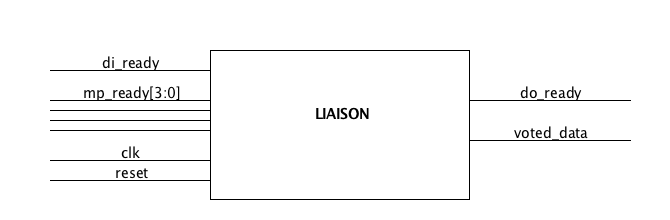
\includegraphics[width=0.5\textwidth]{Figures/ProjectDescription/LiaisonBlackBox}
    \caption{The Liaison module with inputs and outputs (reprinted from \protect\cite{assignment-text}).}
    \label{fig:LiaisonBlackBox}
\end{figure}

Figure \ref{fig:LiaisonBlackBox} shows the Liaison module with the inputs and outputs that are specified for the procject:
\begin{itemize}
    \item \textbf{di\_ready}: A pulse that warns the module that data starts arriving from the microcontrollers. Active high.
    \item \textbf{mp\_data}: input from the microcontrollers. The bus is 4 bits wide, one bit for each microcontroller. The bits arrive serially, with MSB arriving first.
    \item \textbf{reset}: Synchronous reset of the system. Active high.
    \item \textbf{clk}: Clock. All flip-flops are clocked on the positive edge of the clock.
    \item \textbf{do\_ready}: A output pulse that indicates that data starts arriving from the Liasion to the receiver, through the output \textit{voted\_data}.
    \item  \textbf{voted\_data}: The voted result (8 bits) are sent out, clocked and serially, followed by status bits (3 bits) and error correction code (m bits).
        MSB first.
        This can be seen in figure \ref{fig:LiaisonOutput}, where it will take 11+m cycles for a full data package to be sent out. \todo{ "Data packege" might be clumsy, concider revision.}
\end{itemize}

\begin{figure}[h!]
    \centering
    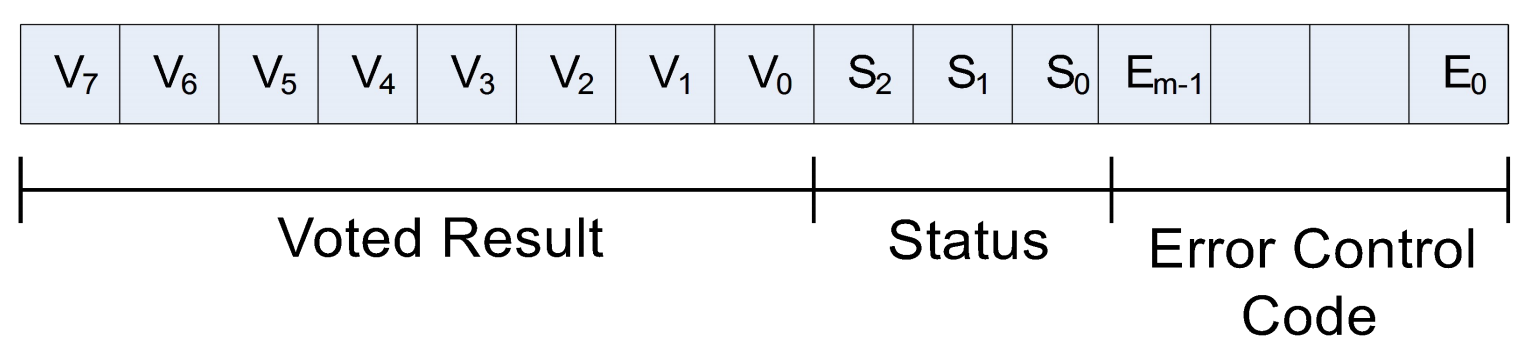
\includegraphics[width=0.5\textwidth]{Figures/ProjectDescription/LiaisonOutput}
    \caption{The total output of data (reprinted from \protect\cite{assignment-text}).}
    \label{fig:LiaisonOutput}
\end{figure}

\begin{figure}[h!]
    \centering
    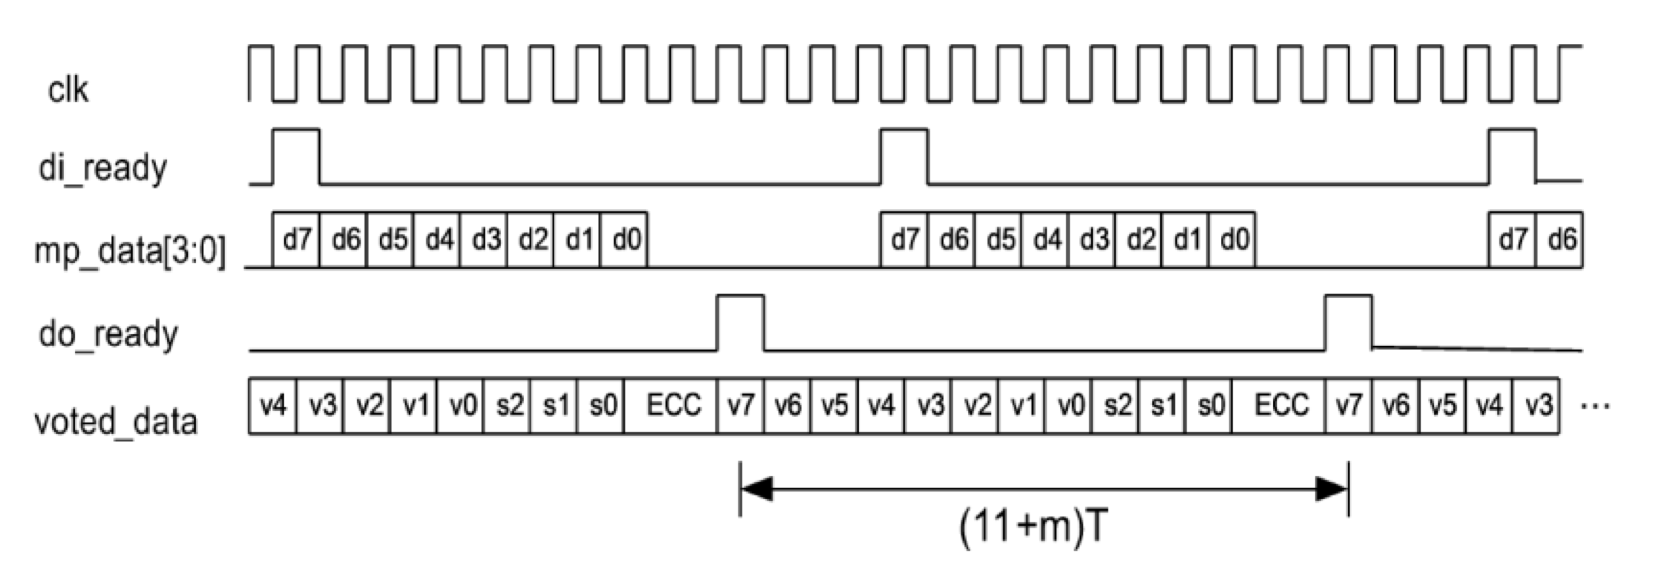
\includegraphics[width=0.5\textwidth]{Figures/ProjectDescription/LiaisonInputOutput}
    \caption{The relationship between the inputs and the outputs of the module (reprinted from \protect\cite{assignment-text}).}
    \label{fig:LiaisonInputOutput}
\end{figure}

Figure \ref{fig:LiaisonInputOutput} shows the system operating with maximum throughput, and it can be seen that there are some delays in the inputs in order to allow the maximum throughput.
Since the Liasion has to send more than just the voted data, it cannot read input data constantly.

\begin{figure}[h!]
    \centering
    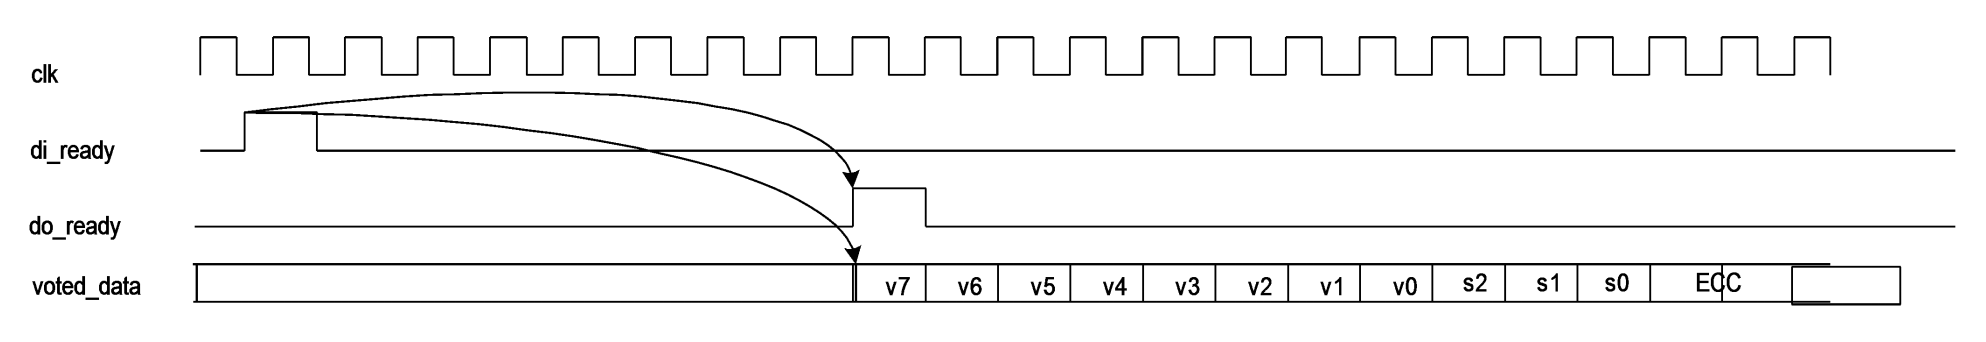
\includegraphics[width=0.5\textwidth]{Figures/ProjectDescription/LiaisonDiReadyDoReady}
    \caption{A pulse of di\_ready causes a do\_ready pulse after n cycles (reprinted from \protect\cite{assignment-text}).}
    \label{fig:LiaisonDiReadyDoReady}
\end{figure}

Figure \ref{fig:LiaisonDiReadyDoReady} shows that there are some delay between \textit{di\_ready} and \textit{do\_ready} that is specified by m cycles.
The latter must be caused by the first, and output data must be sent from the moment \textit{do\_ready} pulses.

\begin{figure}[h!]
    \centering
    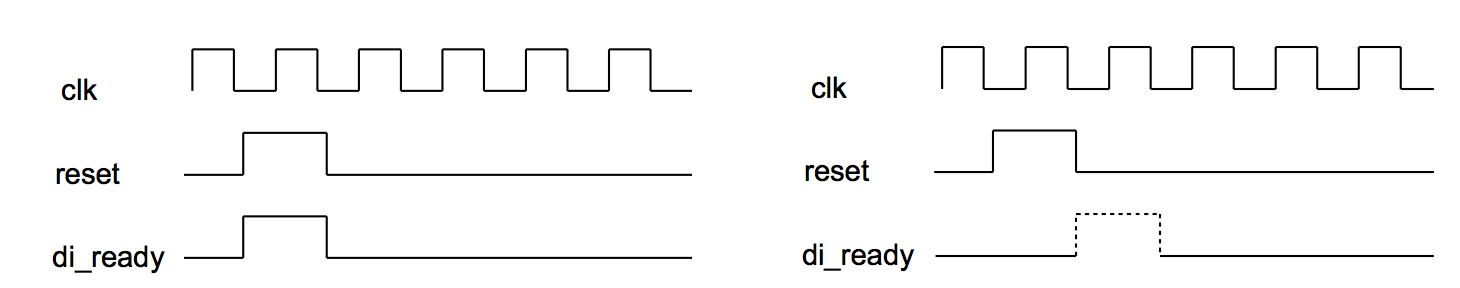
\includegraphics[width=0.5\textwidth]{Figures/ProjectDescription/LiaisonResetDiReady}
    \caption{Reset has precedence over di\_ready (reprinted from \protect\cite{assignment-text}).}
    \label{fig:LiaisonResetDiReady}
\end{figure}

Figure \ref{fig:LiaisonResetDiReady} shows that the \textit{reset} signal must have precedence over the \textit{di\_ready} signal. Liaison must be ready to recieve data immediatly when \textit{reset} is no longer active.

\begin{figure}[h!]
    \centering
    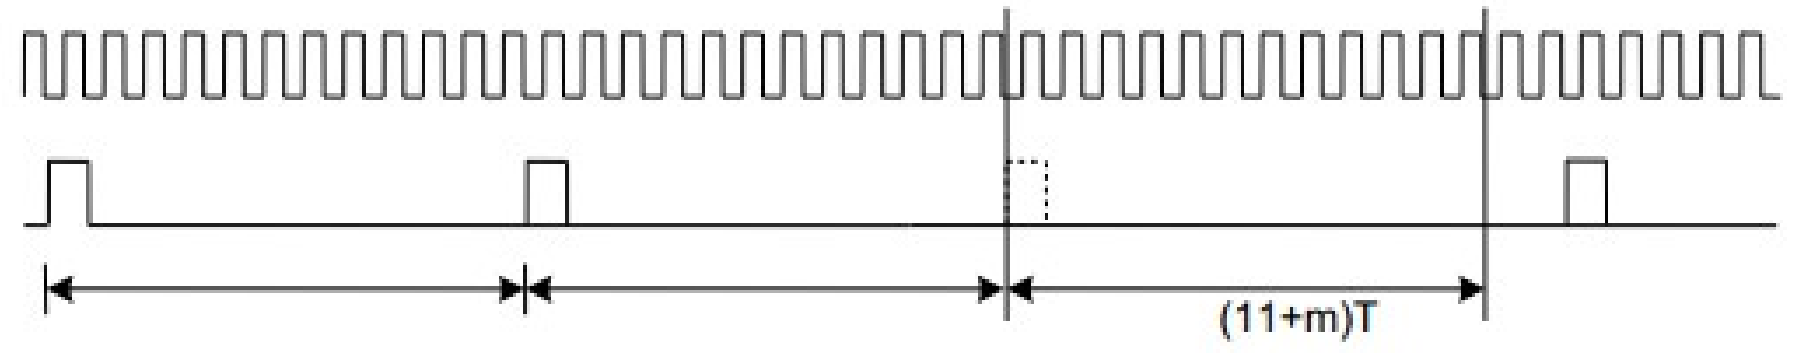
\includegraphics[width=0.5\textwidth]{Figures/ProjectDescription/LiaisonMaxThroughput}
    \caption{The maximum throughput is 11+m, each di\_ready signals may not arrive sooner than that (reprinted from \protect\cite{assignment-text}).}
    \label{fig:LiaisonMaxThroughput}
\end{figure}

Figure \ref{fig:LiaisonResetDiReady} shows the intervals between the pulses of \textit{di\_ready}. The signal may arrive at any time, but there must be at least 11+m cycles between each interval.

\subsection{Project Framework}
The system is to be encoded in VHDL, tested and verified in simulation, and synthesized, with a goal of having a few Look Up Tables (LUTs) as possible. \todo{ Perhaps briefly explain what a LUT is?}
Active HDL \todo{ Version number?} is used for programming in VHDL, as well as creating test benches and running simulations for verification.
Synplify Pro \todo{ Version number?} is used for synthesizing, creating resulting LUTs and estimated frequency, and creating RTL schematics and Gate-Level \todo{ Find correct name} schematics. 
\break 
\todo{ Replace break with new paragraph in such a way that \textit{a)}, \textit{b)}, \textit{c)}, ... is not added}
\break
\todo{ Yes, new paragraph here} The Term Assignment was handed out at \todo{ Insert date here, somewhere in January}. These are the milestones: \todo{ Again, need reference from the Term Assignment}
\begin{itemize}
    \item \textbf{February 18th, 2014}: Assignment 3 of the Course, where the individual One-Bit Voters are designed. They serve as basis of the 8-bit voters
    \item \textbf{February 28th, 2014}: Delivery of technical notes, that will contain preliminary solutions to sub-problems 1, 2 and 3.
    \item \textbf{March 3rd, 2014}: Delivery of Peer Evaluation, containing evaluation of the technical note and project of another group.
    \item \textbf{March 31st}, 2014: Presentation of the project for groups 1-9 (minus 7).
    \item \textbf{April 3rd, 2014}: Presentation of the project for groups 7, 10-19.
    \item \textbf{April 4th, 2014}: Final report delivery.
\end{itemize}


\section{ Solution to the problem.}
\todo{ Term project specifies that the answer to all subproblems is to be explained. We should therefore split these into subsection. }
\subsection{Introduction}
This chapter will explain how the group has implemented the solution for the Term Assignment.
The Term Assignment was split into 5 sub-problems, therefore this report will detail the solution to each sub-problem accordingly.

\todo{ Insert chapter introduction here. Remember to mention that we used Active HDL and Synplify Pro.}
\todo{ WARNING: Points of Term project report specifiaction sort of overlaps. Perhaps own chapters for testing and verification, or only the sub-chapters of this one are enough. Discuss, choose, live, rule, win!} 

\subsection{Sub-Problem 1: State analysis}

The system begins with four working microcontrollers.
As time passes, one by one will fail.
First one microcontroller will fail, and it will be tagged as faulty.
It's input will be disregarded.
The next microcontroller breaks down after more time, and only two will remain.
When a third breaks down, the system will go into shutdown because there are no ways to know which one is correct.
This is implemented as a system state machine, and is illustrated in figure \ref{fig:StateMachine}.
\begin{figure}[h!]
    \centering
    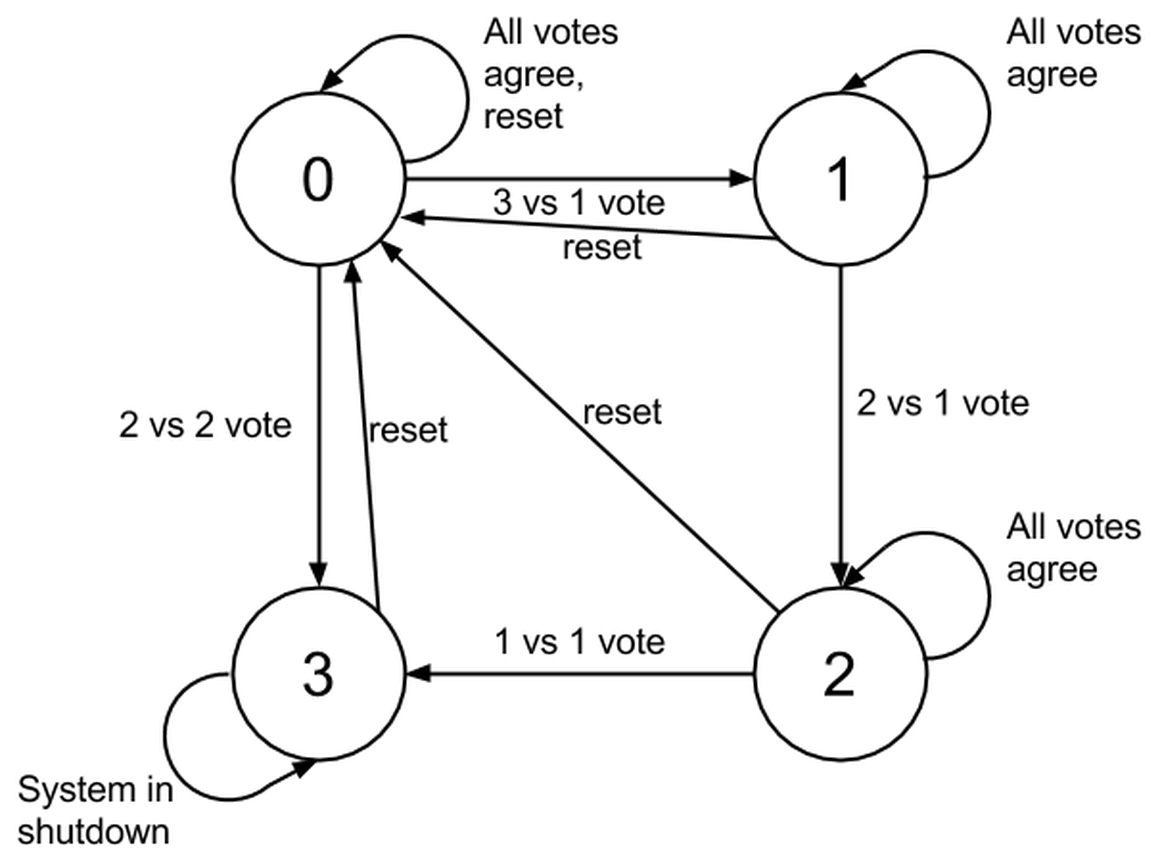
\includegraphics[width=0.5\textwidth]{Figures/Solution/StateMachine}
    \caption{System state machine.}
    \label{fig:StateMachine}
\end{figure}

As long as all microcontrollers agree, no one will be tagged for error and the system will remain in the same state.
For this system, the group has chosen to implement immediate error tagging as soon as an microcontroller disagree with the rest.
Another option could be to not implement error tagging until a series of errors pass and the pattern of errors is recognized.
But a microcontroller should never under any circumstanced disagree with the others as long as it is working, therefore the solution with immediatly error tagging is chosen.
This is also less complex to implement, saving the system for LUTs.
\todo{ This was also the intention of the teachers, given the testbench that was provided. OK to mention?}
As one by one microcontroller fails, they are tagged and the status changes (expected from 0 to 1, 1 to 2 and 2 to 3).
There is also a special case, as can be seen in Figure \ref{fig:StateMachine}:
If two out of the four microcontrollers fail at the same time, the system will go to immediate shutdown, since it can no longer be known which two are working.
The probability for this to happen is very low, but let's say that something unprecedented happens, that damages the satellite (like if it is hit by a small meteorite).
If the damage affects two of the four microcontrollers, so that they disagree, then immediate shutdown would be needed.
The state diagram also shows that when reset occurs, the system returns to the initial state.
A 4-bit register, one bit for each microcontroller, is used to keep record of which microcontrollers work, and which don't.
The 3-bit status bits that the Liasion System sends out will contain data of how many microcontrollers have failed, but not which ones.
Therefore this 4-bit register must be independent of the status output.
Examples are:
\begin{itemize}
    \item \textbf{0000} - All microcontrollers work
    \item \textbf{0100} - Microcontroller \#3 has failed.
    \item \textbf{1010} - Microcontrollers \#2 and \#4 have failed.
\end{itemize}

\subsection{Sub-Problem 2: Design of 1-Bit voter}
Sub-problem 2 concerns the design of the voting system, that will vote one bit at a time.
According to assignments 3 and 4 in the course \todo{ A reference could certainly be useful}, both members of the team were to design a 1-bit voter each, with both in VHDL, simulated and synthesized.

The one-bit voter has the following inputs and outputs:
\begin{itemize}
    \item \textbf{a}, \textbf{b}, \textbf{c}, and \textbf{d}: These are the inputs from the four microcontrollers.
    \item \textbf{clk}: The clock signal for the system
    \item \textbf{reset}: The system reset signal.
    \item \textbf{y}: The one bit voted output.
    \item \textbf{status}: 3 bit status output.
\end{itemize}

The 1-bit voter will implement the state machine as described in the previous section, in order to know the system status and set the status output accordingly.
It will also implement the proposed 4-bit register for error tagging, so that it knows what microcontrollers have failed, and what still works.
It will perform vote at every positive clock edge, by setting the output data accordingly by the majority of the input data.
It will during the voting compare the inputs with the error tag register in order to disregard the correct faulty microcontrollers.
If one of the remaining microcontrollers has an error (by being the minority in the voting process), it is tagged and the system state and status output changes immediatly.
The different status outputs are:
\begin{itemize}
    \item \textbf{000} - All microcontrollers work
    \item \textbf{001} - One microcontroller has failed.
    \item \textbf{010} - Two microcontrollers have failed.
    \item \textbf{111} - System shutdown.
\end{itemize}
If the \textit{reset} signal is activated, the state machine is reset to initial state, the output status is set to 000, and there are not voting until the \textit{reset} signal is no longer active. 

\todo{ Explain test results. Include figures. OR explain in section "Testing and verification" }
\break
\break
\todo{ Explain synthesis results: Estimated Frequency and generated LUTs}
\break
\todo{ Find out if one or both voters must be explained (at least mention synthesis results of the second one). }

\subsection{Sub-Problem 3: 8-Bit voter}

\todo{ Explain test results. Include figures. OR explain in section "Testing and verification" }
\break
\break
\todo{ Explain synthesis results}
\break
\break
The 8-bit voter's main function is to read 8 bits serially from the 4 microcontrollers, and perform voting and error tagging. 
There are several ways of implementing this.

\subsubsection{Options for Architecture}
During the project, the group has discussed and concidered three different alternatives in implementing the 8-bit voter.
For the three alternatives discussed, they all have in common that they are component based implementations, that have at least a Controller Module, and a multiplexer used for selecting output data.
The inputs and the outputs are the same as specified for the Liaison system, and it is possible to use the entire 8-Bit Voter for the entire System, naming it Liaison. 

\begin{figure}[h!]
    \centering
    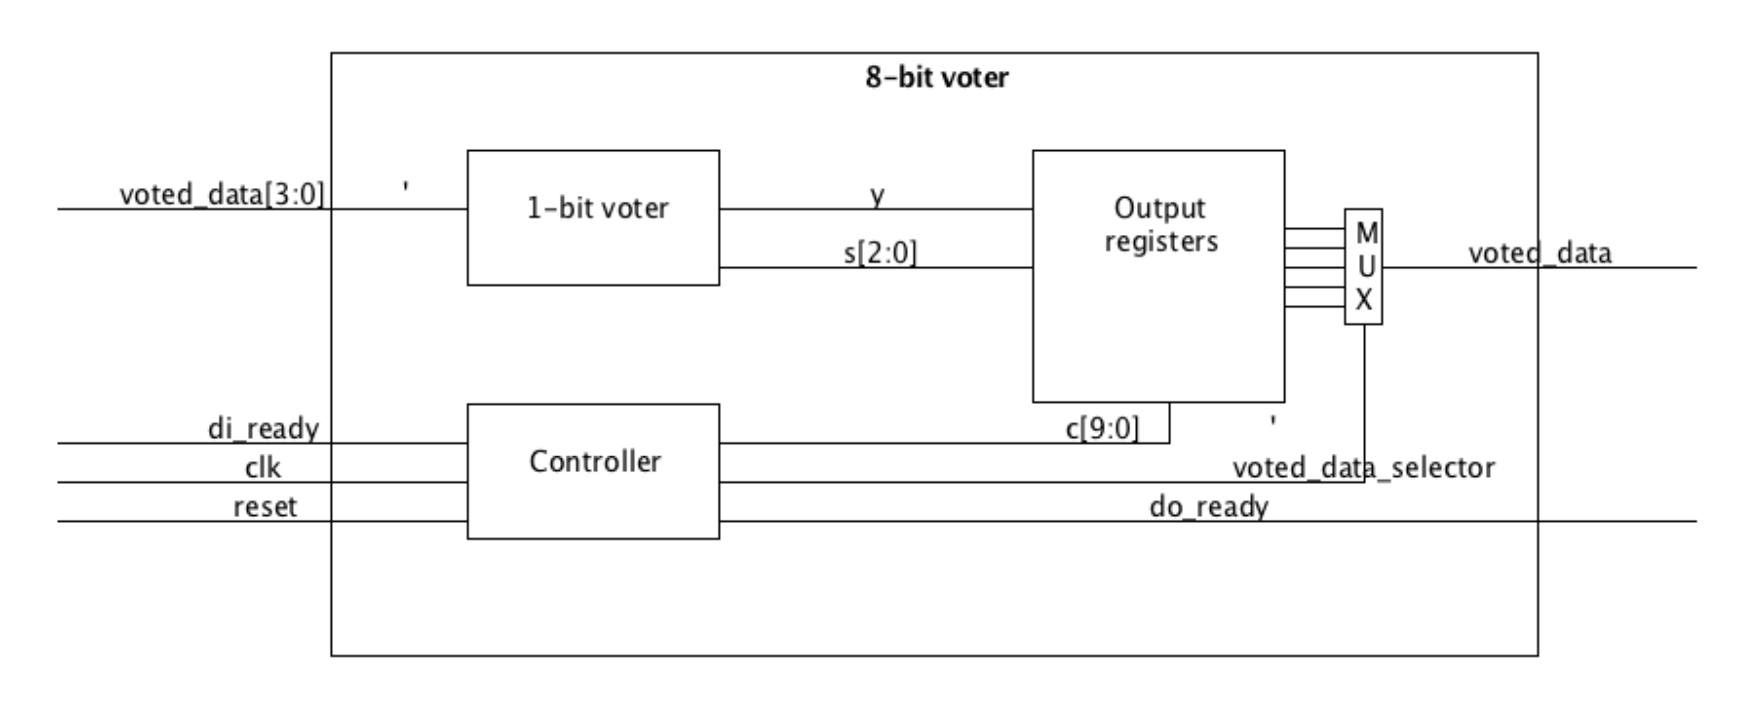
\includegraphics[width=0.5\textwidth]{Figures/Solution/ArchitectureOption1}
    \caption{Optional architecture for the 8-bit Voter: Using 1-bit voter and registers}
    \label{fig:ArchitectureOption1}
\end{figure}
Figure \ref{fig:ArchitectureOption1} shows a component based implementation that includes the 1-bit voter, a controller module, a register module and a multiplexer. Data are received serially, voted serially by the 1-Bit Voter, and the resulting data are stored in registers. After a specified number of cycles, data are to be sent out serially, together with the \textit{do\_ready} signal.
\begin{figure}[h!]
    \centering
    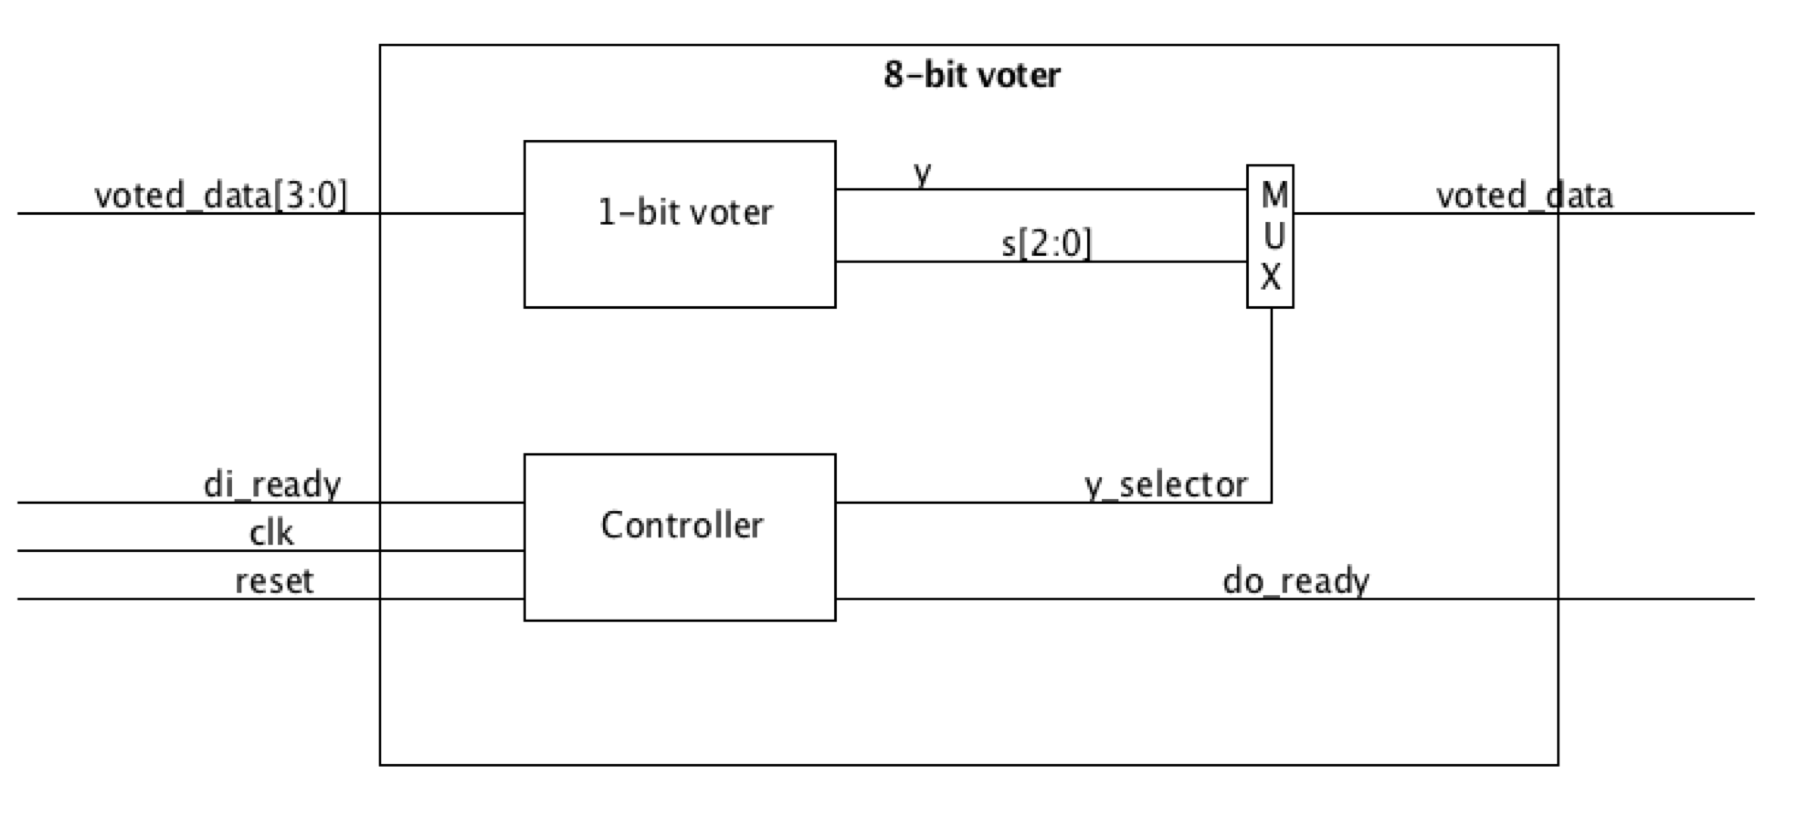
\includegraphics[width=0.5\textwidth]{Figures/Solution/ArchitectureOption2}
    \caption{Optional architecture for the 8-bit Voter: Not using registers}
    \label{fig:ArchitectureOption2}
\end{figure}
Figure \ref{fig:ArchitectureOption2} shows an option where no registers are implemented. 
The idea is to have as small 8-Bit Voter as possible. 
Data that are read and voted serially must be passed on immediatly.

\begin{figure}[h!]
    \centering
    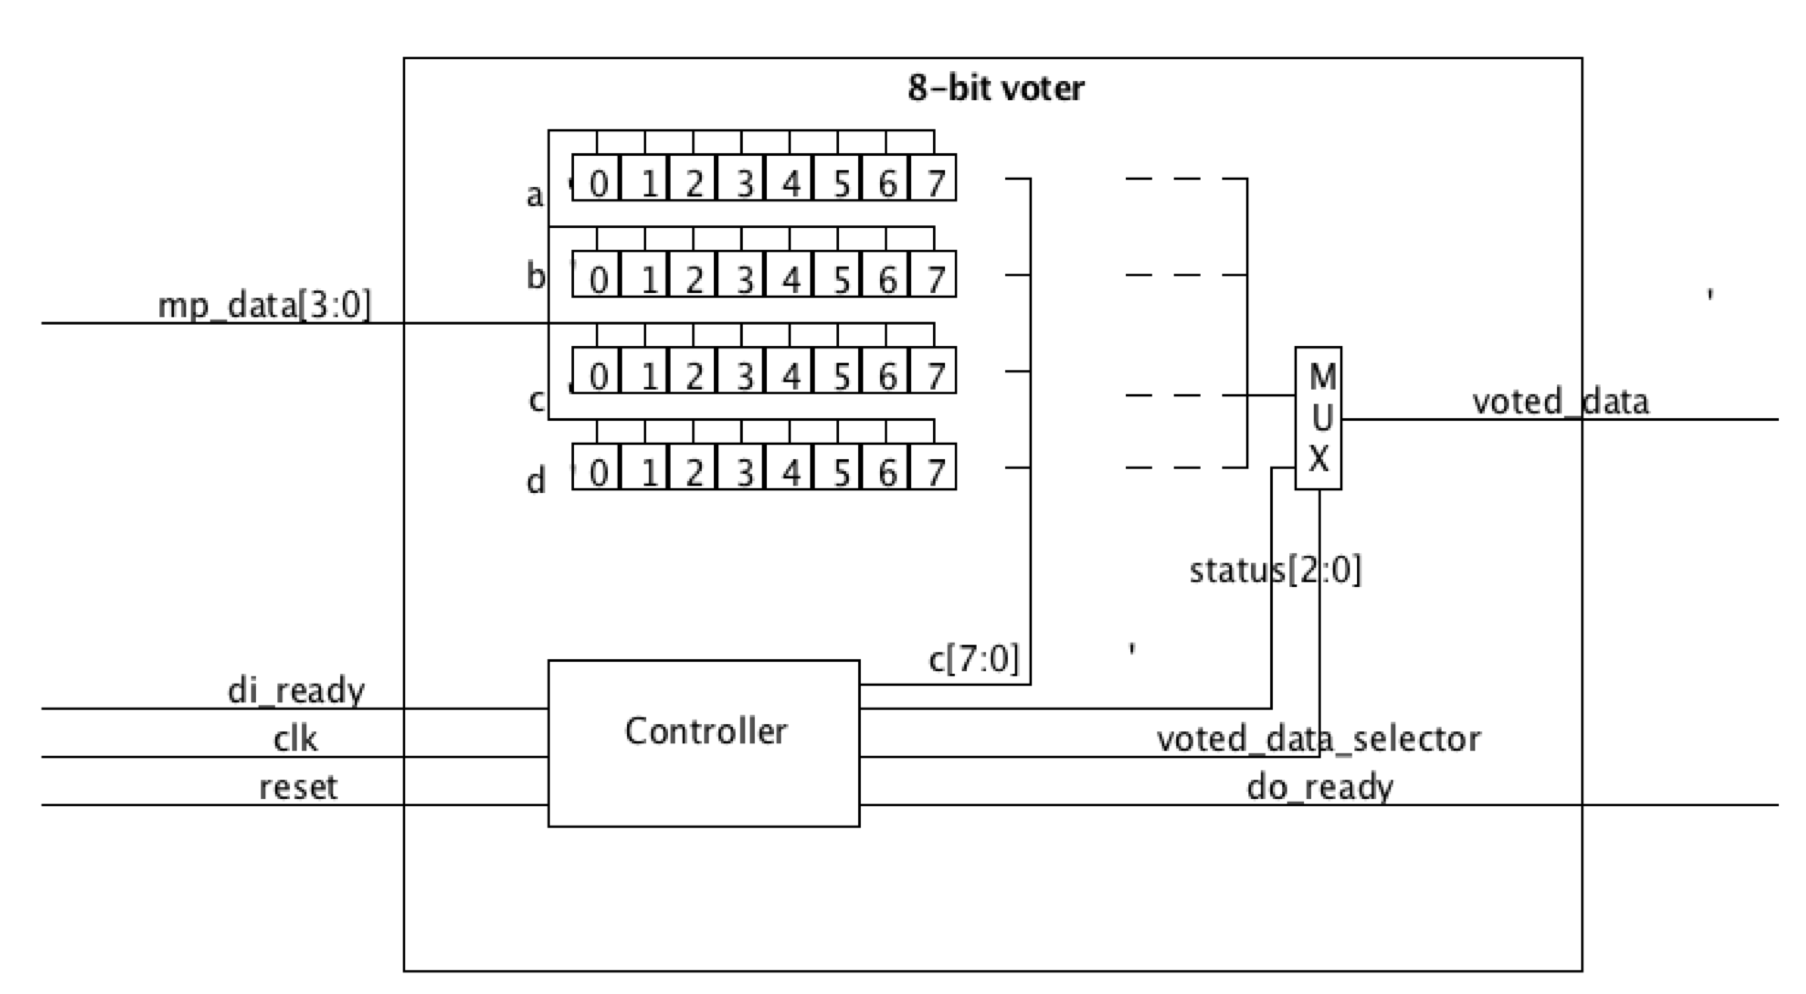
\includegraphics[width=0.5\textwidth]{Figures/Solution/ArchitectureOption3}
    \caption{Optional architecture for the 8-bit Voter: Not using 1-bit voter}
    \label{fig:ArchitectureOption3}
\end{figure}
Figure \ref{fig:ArchitectureOption3} shows an option where the 1-Bit Voter is not used. In this scenario, 4 sets of 8-Bit words are stored and voted.
Though the voting can be done serially for each arrived sets of bits, the idea is that it can also perform instant voting on the entire 8 bit words.
Note that output status data must be handled differently in lack of the designed 1-Bit Voter.
The Controller has this responsibility in this case.

\subsubsection{Choice of Archtecture}
While the second option uses less space than the first one, and it is possible to pass on data immediatly as soon as it arrives, the Term Assignment specifies that the ECC module is to be imeplemented using Hamming Codes.\todo{ This is currently the first time Hamming Code is mentioned. Perhaps define earlier?} 
The ECC calculation cannot be done before all data have \todo{ "Have" or "has" when using the word data?} arrived, voting is done and the status bits are updated.
But with this implementation, the data is sent immediatly, but not stored.
The ECC module will have to implement registers, but this contradicts the idea behind this option of not using registers.
The second option is thus not compatible with expanding the system with an ECC module.
\break
The third option uses another solution than a 1-Bit voter, but the group conciders the 1-Bit Voter to be sufficient.
Implementing another voter is concidered a waste of time since there is already a solution available, that the group conciders to be good enough.
All data arrives serially, and are sent out serially from the Liasion, and serial voting between receiving and sending is sufficient.
If all received data were to be voted instantly by voting the entire word, it would create constriction on receiving data and sending out data.
Only status data or ECC data from the previous vote can be sent out while an 8-bit voting is performed.
Though maximum throughput is possible, the design is more difficult to implement.
This solution is likely to have greater complexity than the first option, and the use of four sets of registers make the 8-Bit Voter conciderably larger than the first option.
Given these premises, the group has chosen to implement the first option, since the other options are concidered weaker.
The full architecture, which includes the ECC module, can be seen in figure \ref{fig:ArchitectureFinal}. Note that this is named Liasion, since it is used as topmodule for the Liasion system.

\begin{figure}[h!]
    \centering
    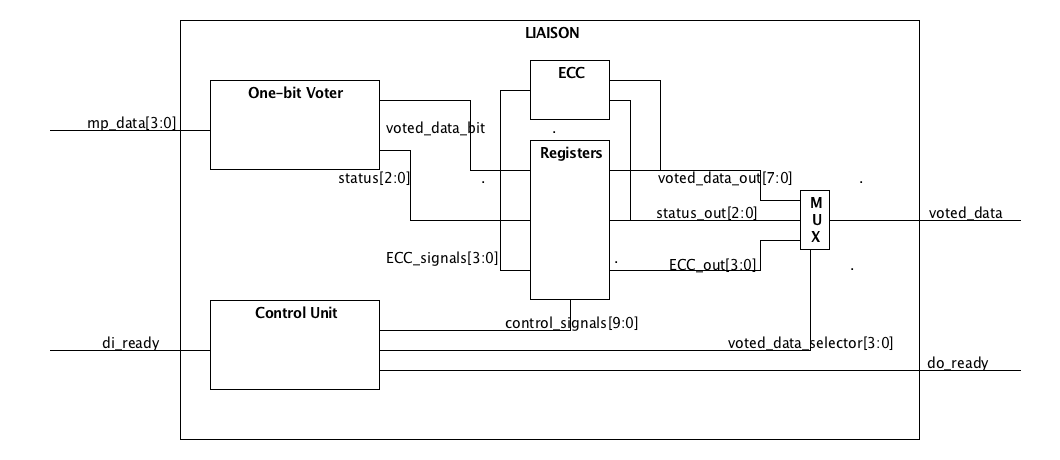
\includegraphics[width=0.5\textwidth]{Figures/Solution/ArchitectureFinal}
    \caption{Chosen architecture for the 8-bit Voter}
    \label{fig:ArchitectureFinal}
\end{figure}

\subsubsection{The Register Module}
\begin{figure}[h!]
    \centering
    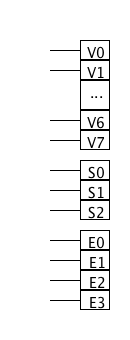
\includegraphics[width=0.10\textwidth]{Figures/Solution/Registers}
    \caption{Implemented registers}
    \label{fig:Registers}
\end{figure}
Figure \ref{fig:Registers} shows the contents of the register modules.
There are 8 registers for storing voted data and 3 for storing status data from the 1-Bit Voter.
The group has chosen to implemen 4 bits of ECC data in this project.
The register module is controlled by a 10-bit control\_signal, that is used when storing data.
The control\_signal, which is set by the control\_unit, has 1 bit for every 8 voted data register, since voted data arrive serially and must be stored one by one.
The 9th bit is used for storing data in the status registers, since all 3 status bits arrive simultaniously.
The 10th bit is used for storing data in the ECC registers, since ECC data are calculated and thus stored thenext  cycle after being done with all voted data and status data.
If none of these control bits are active, no new data will be stored.

\subsubsection{The Controller Module}
The Controller Module is responsible for controlling the registers when storing data, and setting the multiplexer so that correct data is sent out.
The module is implemented as two state machines.
The first is activated by the \textit{di\_ready} signal, and sets the 10-bit control\_signal that is connected to the register module.
After a specified number of cycles, in this case 7, the \textit{do\_ready} pulses for one cycle.
The second state machine is activated by the \textit{do\_ready} signal, and is responsible for setting the 4-bit voted\_data\_selector that is connected to the multiplexer, so that data from the registers are sent out in the correct order.
There are 7 cycles before activating the second state machine, and 15 (11+m) cycles for the second state machine for setting the output data. 
In total this makes up 22 cycles \todo{ Count in test} before going idle, should there be no more \textit{di\_ready} signals.
If the next \textit{di\_ready} signal arrives too early, it will have to be ignored, since the shortest possible intervals for the syste are 15 cycles.

\todo{ Concider implementing figures with the stateMachines.}

\subsection{Sub-Problem 4: Error Correction Circuit}
\todo{ Explain how the ECC is implemented, perhaps explain Hamming Coding. Include figure (screenshot it from the presentation). }
\break
\break
\todo{ The term project states: "Your final report should comment on the use of intellectual property-modules and the reasoning behind why this scheme is appropriate." To this.}
\break
\break
\todo{ Explain the alternative of using 8 bits, possible pros, and the cons that were the reason for choosing 4 bits instead} 
\break
\break

\todo{ Explain test results. Include figures. OR explain in section "Testing and verification" }
\break
\break
\todo{ Explain synthesis results}

\subsection{Sub-Problem 5: Analysis of error probabilities}
A microcontroller is expected to fail on an avarage of 6 years.
Sub-Problem 5 of the Term Assignment specified that 3 mathematical expressions on failure after a time \textit{t}, as well as Mean Time To Failure (MTTF) for the system are to be calculated:
\begin{itemize}
    \item The probability for error in maximum one controller (that is zero or one) after \textit{t} time. This will be expressed as P(Max(1)). 
    \item The probability for error in maximum two controllers after \textit{t} time. This will be expressed as P(Max(2)).
    \item The probability for error at least three controllers after \textit{t} time. This will be expressed as P(Least(3)).
    \item The MTTF for the whole system.
\end{itemize}

The propability that a machine does not fail after a time \textit{t}, given the expected life time \textit{T}, is expressed as $P = P(t) = e^{-t/T}$.
Since the expected life time for a microcontroller is T = 6, the probability is expressed as $P = P(t) = e^{-t/6}$. 
The different probabilites that are calculated are:
\begin{itemize}
    \item $P(Max(1)) = e^{-t/2}+3(e^{-t/2}-e^{-2t/3})$
    \item $P(Max(2)) = 3e^{-2t/3}-8e^{-t/2}+6e^{-t/3}$
    \item $P(Least(3)) = 1-3e^{-2t/3}+8e^{-t/2}-6e^{-t/3}$
    \item MTTF = 6.5 years.
\end{itemize}

These calculations and how they are done are explained in full details in Appendix C.

\todo{ Refer properly to Appendix C.}

\section{ Testing and verification }
\todo{ Either explein the testing and verification here, or do it seperately in the subchapters of the previous chapter. Delete this chapter if we choose the other solution. I vote this one. But if we do so, for consistensy we may then have to create a independent chapter for Synthesis }
\subsection{ Introduction}
The Liasion System, with all it's components, are to be throuthoroughly tested by simulating the behaviour and ensuring that desired behaviour occurs.
Whenever an error in behaviour has occured, the VHDL code for the component has been modified in order to remove the error.
After completing synthesis in Synplify Pro, the group redid the tests in Sythesis Simulation in Active HDL, which do the tests with any changes that might have occurred after synthesizing the project. 
This section will present what were tested in each component, and the final test results.

\subsection{ Tests and verification of 1-Bit Voter}
Originally, each member of the group created a test bench of their own for their 1-Bit Voters, as part of assignment 3.
The group later received a test bench from the course staff for the evaluation of assignment 3, and this has replaced the old test benches.
The reason behind this choice is that the group conciders the scenario \todo{ Find better word than scenario?} in the test bench to be realistic for all situations.
It is not likely that there will arise other situations when it comes to inputs and behaviour of the module as is tested in this test bench.
Therefore the group conciders this test bench to do full coverage of the 1-Bit Voter.
The test bench compares outputs with expected results, and throws an error whenever there is a difference between test outputs and expected outputs.
Different combinations of inputs are tested, and one by one microcontroller are set to fail.
The failed microcontrollers are tested for error tagging by testing whether their data has any affection on the output \textit{voted\_data}.
\textit{Reset} is always activated to reset and test for other input combinations.
The entire test passes with the current 1-Bit Voter. 
\todo{ Explain test results. Include screenshot (Uh... the provided test bench is not of that kind).}

\subsection{ Controller Module}
The Controller Module is tested for these different situations:
\begin{itemize}
    \item \textbf{Long intervals between \textit{di\_ready}}. 
    The controller should set it's outputs so that only the one stream of input data associated with the received \textit{di\_ready} signal should be stored and sent out of the Liasion module.
    This is seen in the test as changes in the outputs of the module.
    These changes should be traversed only once per \textit{di\_ready}, and is expected to last for 22 \todo{ Count in test} cycles.
    \item \textbf{Too short intervals between \textit{di\_ready}}.
    The controller should ignore \textit{di\_ready} signals that arrive too early, since the system is not finished receiving and/or processing the current data.
    \item \textbf{Maximum throughput}.
    The controller should enable maximum througput when \textit{di\_ready} signals are received every 15 cycles.
    This can be seen as there are changes on the output \textit{voted\_data\_selector} at every clock cycle.
    \item \textbf{Reset}.
    Whenever the \textit{reset} signal pulses, the controller should synchronously halt any activity, and reset both state machines and outputs to initial value.
    Any waiting \textit{do\_ready} signal should not be sent out.
    Reset is tested for both before activating second state machine, and after. 
\end{itemize}
These are the different situations that might occur for the controller module, therefore this test is concidered to give full coverage for the controller module.
\todo{ Include screenshot from test. Explain results}

\subsection{ ECC }
\todo{ Explain choice of test bench. Explain why only partial coverage is enough. }
\break
\break
\todo{ Explain test results. Include screenshot. }

\subsection{ Liaison }
The test bench for the Liaison system is a test of the top level.
The behaviour of the Liaison relies heavily on the 1-Bit Voter and the Controller Module.
These two components are already tested in full coverage, therefore most of the Liasion is indirectly tested.
The test bench gives thus only partial cover, only to do a small control to ensure that the components and the toplevel cooperate as expected.

\begin{figure}[h!]
  \centering
      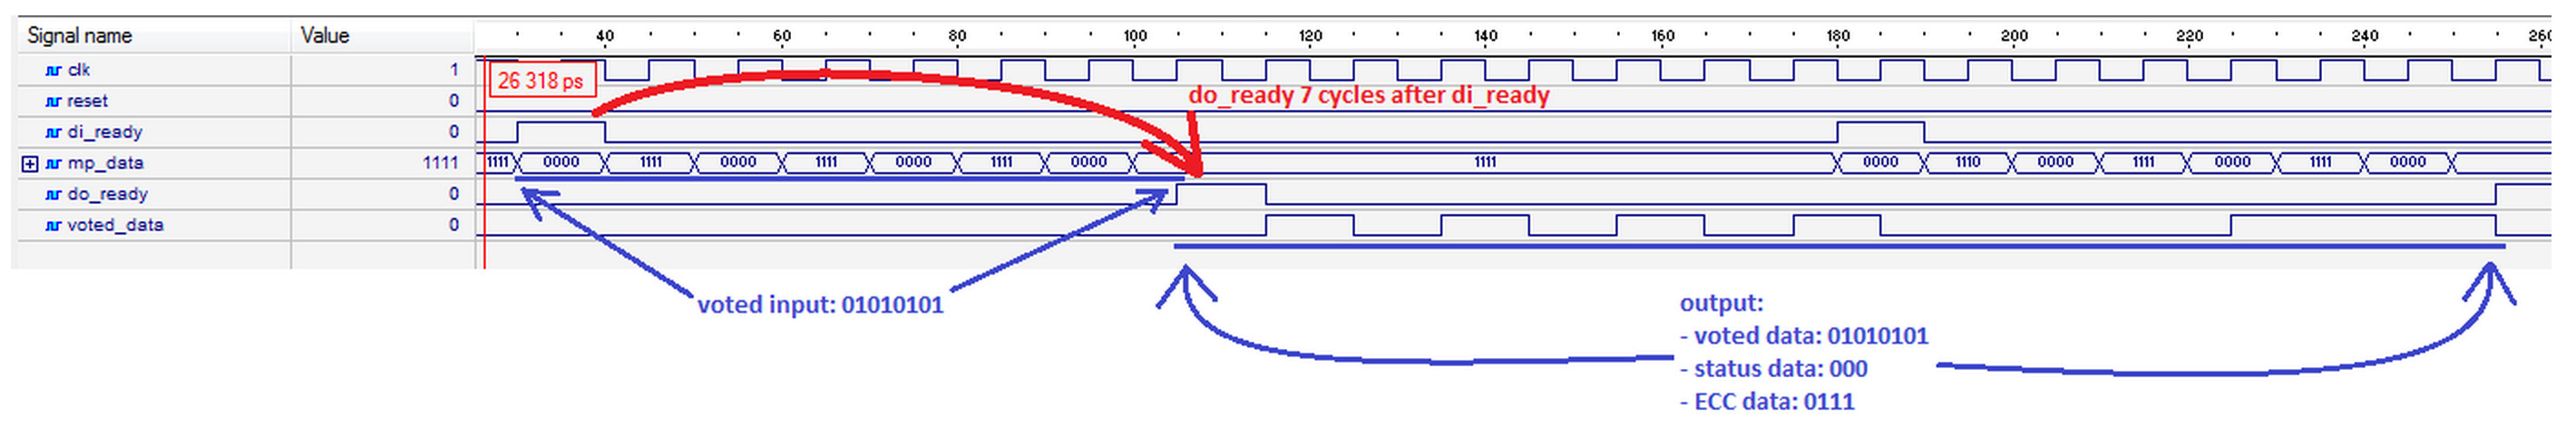
\includegraphics[width=0.5\textwidth]{Figures/Tests/LiaisionTest}
  \caption{Screenshot from Liaison Test}
  \label{fig:LiaisonTests}
\end{figure}

Figure \ref{fig:LiaisonTests} shows a screenshot of the test output.
The red arrow marks the interval between the \textit{di\_ready} and the \textit{do\_ready}, illustrating that the first activates the second.
The inputs are also markes, and are sent out as the 8 first bits of the output.
The output also includes status bits and ECC bits.
The output of this tests show that the components cooperate as expected.
This depends on that each component works as expected, but that is already tested in the other test benches.

\section{Synthesis }
\todo{ Decide whether we should have a own chapter for this or not. If we choose this option for testing and verification, we should do this for synthesis as well in the name of consistency. }
\break
\break
\todo{ Insert introduction }
\break
\break
\todo{ Refer to Appendix B for schematics. Both RTL and that other one. }

\section{Feedback and other Information}
\todo{ The teachers wanted feedback. They also want to know the time spent on the work. This is where it should be added}.
\subsection{Feedback}
\todo{ The cake is a lie!}

\subsection{Time spent}
\todo{insert details of how much time spent on the project, including on this report.}

\section{Conclusion}
\todo{ Compulsory. Have a good wrap up, somehow. }

\section{Acknowledgements (optional)}

Indiana Jones. Should also mention group 2 and the student assistant.

\section{ Other problems/needs to be solved:}
\subsection{ Appendixes}
\todo{ Appendix A: Project codes }
\break
\break
\todo{ Appendix B: Synthesis Schematics. Both RTL and that other type, propose top architecture first then One-bit-Voter, Controller, Registers and ECC. RTL first then that other type.}
\break
\break
\todo{ Appendix C: The Probability Calculation. I got it covered. }
\subsection{ Other problems/needs:}
\todo{ Find out where to list up time spent in the project.}

\bibliography{bibliography}
\bibliographystyle{plain}
\nocite{*}

\clearpage
\begin{titlepage}
    \newcommand{\HRule}{\rule{\linewidth}{0.5mm}} % Defines a new command for the horizontal lines, change thickness here
    \center % Center everything on the page
    \vspace*{3cm}
    \HRule \\[0.4cm]
    { \huge \bfseries Appendices}\\[0.4cm] % Title of your document
    \HRule \\[1.5cm]
\end{titlepage}
\clearpage
\begin{titlepage}
    \newcommand{\HRule}{\rule{\linewidth}{0.5mm}} % Defines a new command for the horizontal lines, change thickness here
    \center % Center everything on the page
    \vspace*{3cm}
    \HRule \\[0.4cm]
    { \huge \bfseries Appendix A}\\[0.4cm] % Title of your document
    \HRule \\[1.5cm]
\end{titlepage}
%\includepdf[pages={1}]{Appendixes/AppendixA.pdf}
\clearpage
\begin{titlepage}
    \newcommand{\HRule}{\rule{\linewidth}{0.5mm}} % Defines a new command for the horizontal lines, change thickness here
    \center % Center everything on the page
    \vspace*{3cm}
    \HRule \\[0.4cm]
    { \huge \bfseries Appendix B}\\[0.4cm] % Title of your document
    \HRule \\[1.5cm]
\end{titlepage}
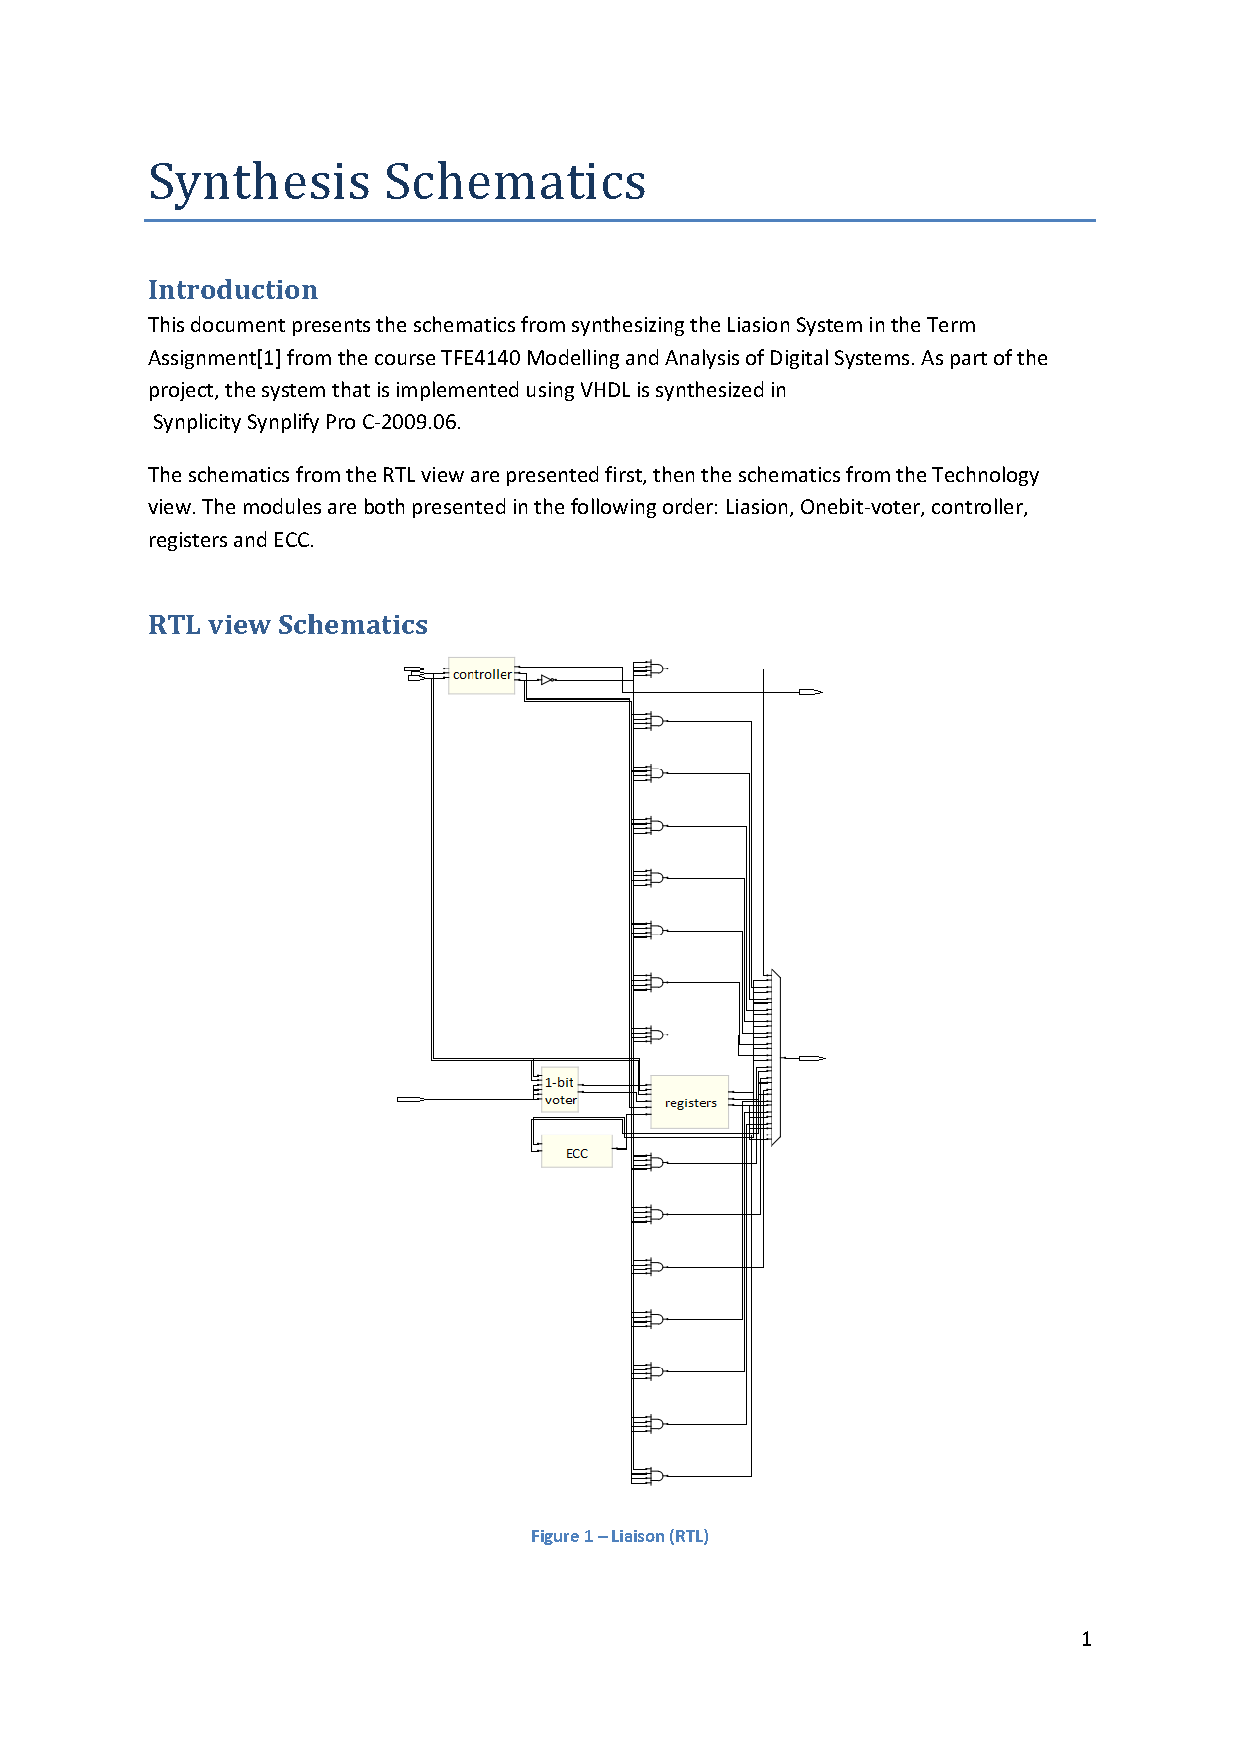
\includepdf[pages={1,2,3,4,5,6,7,8}]{Appendixes/AppendixB.pdf}
\clearpage
\begin{titlepage}
    \newcommand{\HRule}{\rule{\linewidth}{0.5mm}} % Defines a new command for the horizontal lines, change thickness here
    \center % Center everything on the page
    \vspace*{3cm}
    \HRule \\[0.4cm]
    { \huge \bfseries Appendix C}\\[0.4cm] % Title of your document
    \HRule \\[1.5cm]
\end{titlepage}
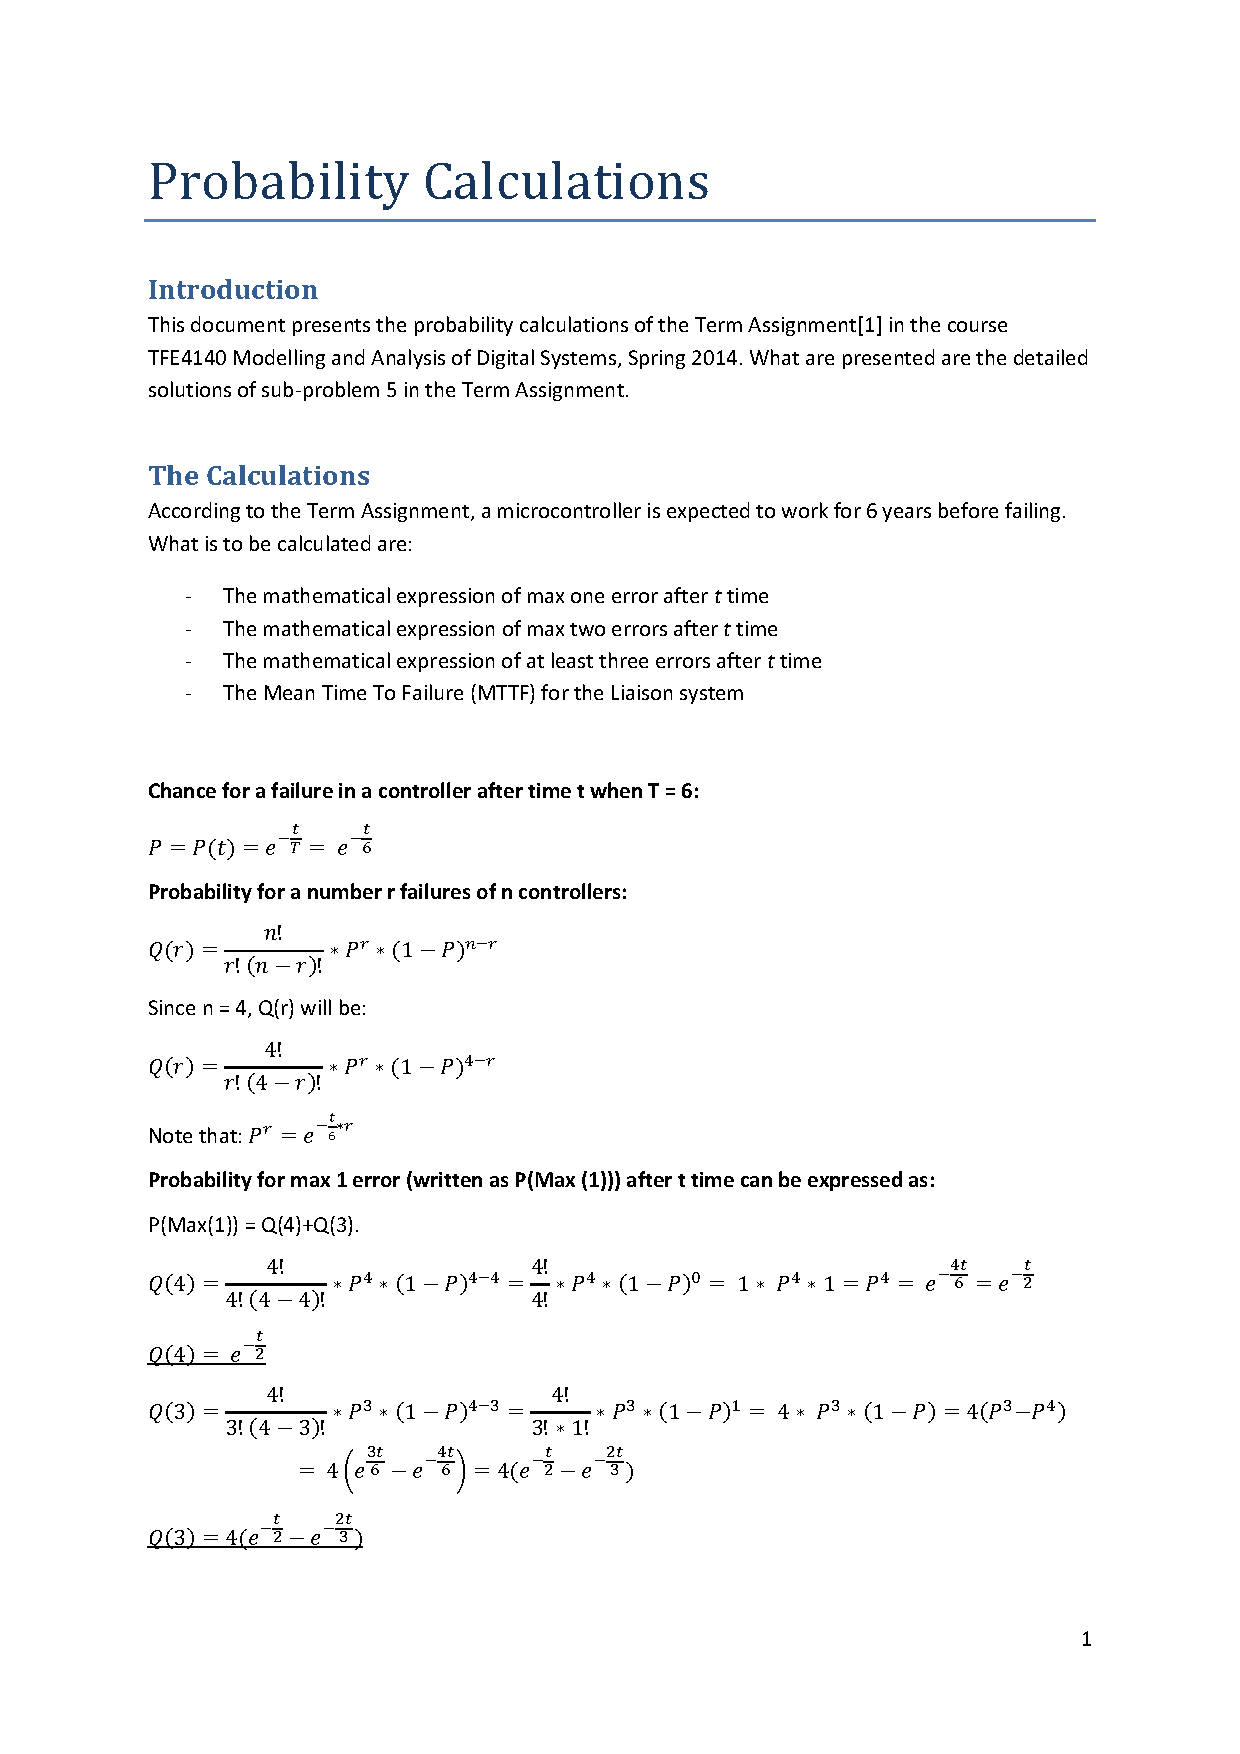
\includepdf[pages={1,2,3,4}]{Appendixes/AppendixC.pdf}

\end{document}
